\chapter{Analysis of the density of charge}

To evaluate the spatial distribution of carriers before the quantum population regime, a two-dimensional slice of the electron charge density $n$ is extracted at the coordinate $Z = 45\text{ nm}$. This specific height is crucial as it accurately cuts through the active silicon channel where the double quantum dot is designed to form.

\begin{figure}[htbp] 
    \centering 
    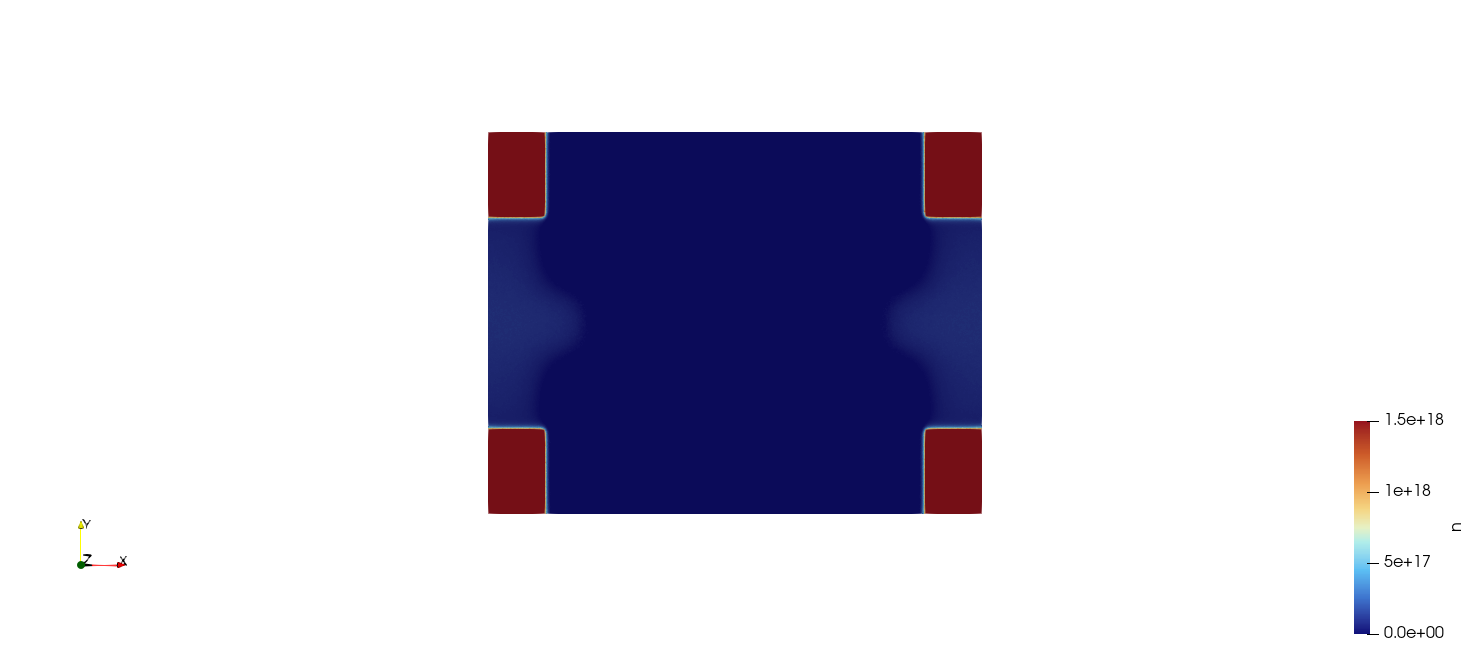
\includegraphics[width=0.8\textwidth]{Images/Nfile/Slice_file_n_lab5.png} 
    \caption{Slice at Z = 45 of the file n.}
    \label{fig:mia_immagine_1} 
\end{figure}

As shown in the 2D density map in Fig.~\ref{fig:mia_immagine_1}, the central region of the channel is completely depleted of electrons. This behavior is directly governed by the electrostatic action of the lateral barrier gates. These gates have a direct influence on the behavior of the reservoirs and the two dots: in fact, the shape of the Drain and the Source, represented by the light blue regions at the extremities of the photo, exhibits a small protrusion towards the center, which is tightly constrained from both below and above along the Y-axis. This is the direct effect of the Y-gates, which are strictly required to achieve electrostatic confinement for the quantum dots along the Y-direction as well. Consequently, the carriers can only communicate with the central dots by tunneling through the narrow potential barriers.A distinctive feature of the density map is the presence of four highly populated regions located at the corners of the domain, highlighted in dark red due to their maximum electron density values. The inclusion of these highly doped $n$-type zones is crucial for the operation of the device at cryogenic temperatures ($10\,\text{mK}$). At such extreme temperatures, standard silicon undergoes the phenomenon of \textbf{carrier freeze-out}, losing its conductivity and turning into an insulator. This would prevent the formation of proper ohmic contacts with the external metal lines due to the creation of insurmountable Schottky junctions.To bypass this limitation, these four corner regions are heavily doped with $n$-type impurities, shifting the material into a degenerate state where it behaves like a metal, maintaining a high and stable concentration of free electrons even at millikelvin temperatures. These zones act as intermediate electron reservoirs connected to the external contacts. When the gate voltages are applied, these highly conductive corners ensure that carriers can be readily supplied to the classical Source and Drain extensions (the light blue horizontal channels) and, subsequently, tunnel into the central quantum dots.
To quantitatively validate these 2D observations, a 1D Plot Over Line was performed across the symmetry axis at $Y = 136.5\text{ nm}$.

\begin{figure}[htbp] 
    \centering 
    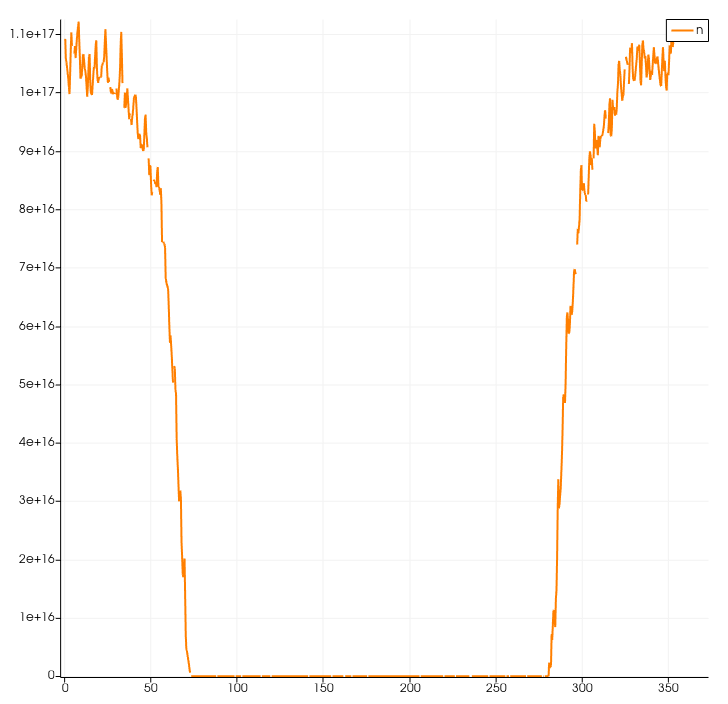
\includegraphics[width=0.8\textwidth]{Images/Nfile/Plot_file_n_lab5.png} 
    \caption{Plot overline at Y = 136.5 of the file n.}
    \label{fig:mia_immagine_2} 
\end{figure}

The 1D profile provides a clear confirmation of the assumptions made before: the electron density reaches its maximum values at the opposite extremes of the domain, marking the horizontal Source and Drain reservoirs cut by the line. Specifically, we can notice that this maximum concentration is on the order of $10^{17}\,\text{cm}^{-3}$, which represents a high value, yet remains lower than the peak concentration of $10^{18}\,\text{cm}^{-3}$ previously observed in the degenerate corner regions. Conversely, the density drops sharply and remains strictly zero throughout the entire central core. This confirms that the electrostatic landscape successfully isolates the quantum dot region from classical drift-diffusion currents, establishing the ideal zero-background environment required for single-particle Schrödinger-Poisson simulations.